%!TEX root = ./nips_2018_sketchmcmc.tex

\section{Experiments}

\begin{figure}
\subfigure[]{
	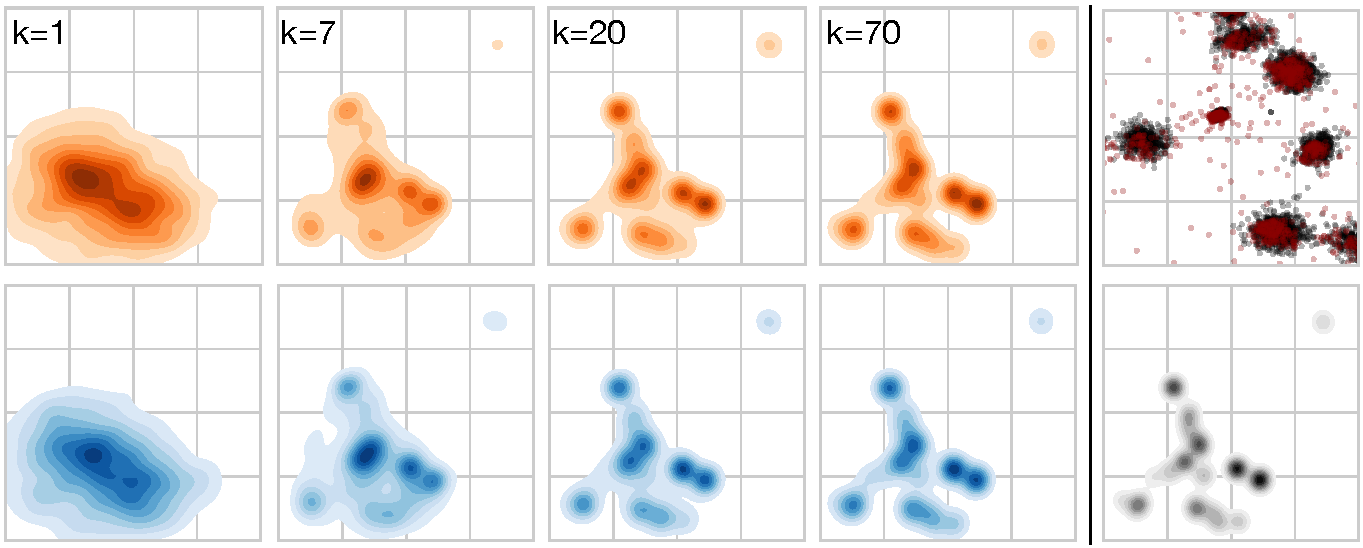
\includegraphics[width=0.65\columnwidth]{figures/gmm_iter.pdf}
	\label{fig:toy_example}
} \hfill
\subfigure[]{ 
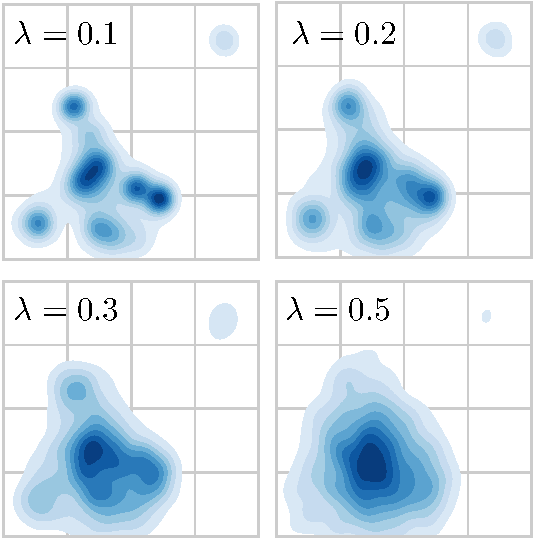
\includegraphics[width=0.255\columnwidth]{figures/gmm_reg.pdf}
\label{fig:lambda_supp}
 }
 \vspace{-\baselineskip}
\caption{a) \textbf{Left:} the distribution of particles (contour plots) during the estimation-stage (top) and prediction-stage (bottom). \textbf{Right:} (top) close-up of some generated particles in red superimposed with data points in black, (bottom) target distribution. b) Influence of the regularization parameter $\lambda$. }
\end{figure}

%I think the real procedure is not helping anything computationally and making the presentation a bit confusing. 
In this section, we evaluate the SWF algorithm on both synthetic and real data settings. In all cases, the initial distribution $\mu_0$ is selected as the standard Gaussian distribution on $\R^d$, we take $Q=100$ quantiles, which proved sufficient to approximate these functions faithfully, and we have observed that $N=3000$ particles are sufficient. 

% \footnote{}


% In this section, we evaluate the SWF algorithm on both synthetic and real data settings. In all cases, the $N$ initial particles $\bar{X}^i_0\in\mathbb{R}^d$ are obtained by first drawing i.i.d.\ standard Gaussian $\bar{Z}^i\in\mathbb{R}^m$ with $m\ll d$. Then we generate random matrix $A$ of size $d\times m$, and finally set $\bar{X}^i_0=A\bar{Z}^i$. This results in $\mu_0=\mathcal{N}(0,AA^\top)$. %This procedure allows us to use the with an arbitrary input dimension.

% \subsection{Toy example: multivariate Gaussian Mixture Model}
% \label{sub:toy_example}

\begin{wrapfigure}{R}{0.40\textwidth}
\vspace{-10pt}
\begin{centering}
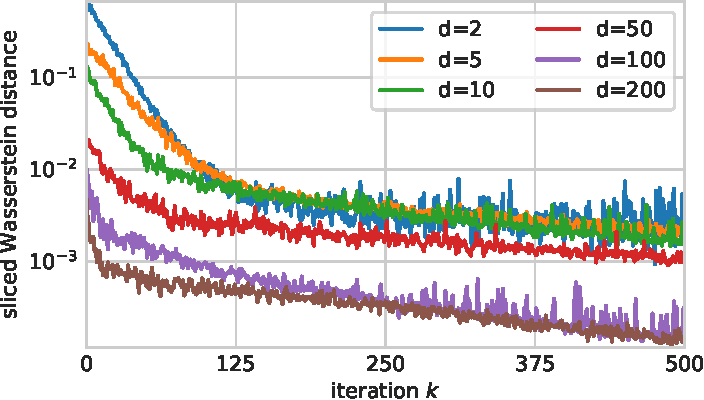
\includegraphics[width=0.40\columnwidth]{figures/SW2_cost-crop.pdf}
\par\end{centering}
\caption{Approximately computed $\SW$ between output $\bar{\mu}_{k}^{N}$ and data distributions $\nu$ in the toy example GMM case for different data dimensions $d$.
\label{fig:toy_sw}}
\vspace{-10pt}
\end{wrapfigure}
\textbf{Gaussian Mixture Model: }
We perform the first set of experiments on synthetic data where we consider a standard Gaussian mixture model (GMM).
%
We set the number of the mixture components to $20$ and for each component we randomly draw the weight, covariance matrices and centroids. We make sure that the centroids are sufficiently distant from each other in order to make the problem more challenging. Given the model parameters, we generate $P=50000$ data samples in each experiment.


In our first experiment, we set $d=2$ for visualization purposes and illustrate the general behavior of the algorithm. Figure~\ref{fig:toy_example} shows the evolution of the particles through the iterations. Here, we set $N_\theta=30$, $h=1$, and $\lambda=10^{-4}$.
%
We observe that the empirical distribution of the particles converges rapidly to the target distribution. Furthermore, we can see that the QF, $F^{-1}_{\theta^*_\#\bar{\mu}_{kh}^{N}}$ that is computed with one set of particles (so-called the \textit{estimation} stage) can be perfectly re-used for new unseen particles in a subsequent \textit{prediction} stage. In both cases, we observe two remarkable outcomes: (i) Even when some modes are isolated from the others, SWF is able to capture them successfully and we never observe a mode collapse. This is due to the OT nature of the procedure. (ii) The generated particles do not collapse on the data, thanks to the entropy regularization.

In our second experiment, we investigate the effect of the level of the regularization. We use the same setting as the previous experiment, whereas we differ the value of $\lambda$ and run the algorithm for sufficiently many iterations. As we can observe from Figure~\ref{fig:lambda_supp}, the distribution of the particles becomes more spread with increasing $\lambda$. This is due to the increment of the entropy, as expected.

% There, the target distribution is displayed on the rightmost panel, as obtained through a contour plot of the data samples. On the left panel, we see the output distribution of the SWF at different iterations. 


In our next experiment, we investigate the behavior of the algorithm for varying dimensionality $d$. Since visualizing the results becomes non-trivial for large $d$, in this experiment we directly monitor the (approximately computed) $\SW$ distance between the distribution of the particles and the data distribution. Even though minimizing this distance is not the real objective of our method, arguably, it is still a good proxy for understanding the convergence behavior. 
%
Figure~\ref{fig:toy_sw} illustrates the results. We observe that, for all choices of $d$, we see a steady decrease in the cost for all runs, which is in line with our theory. Since we used the same $\lambda$ for all $d$, the entropy term becomes relatively stronger in the case of smaller $d$, which results in larger $\SW$. This advocates the use of larger $\lambda$ as the dimensionality increases. 




% Our next experiment aims to assess whether SWF achieves its objective of decreasing the sliced Wasserstein distance between the output $\bar{\mu}_{k}^{N}$ and the target $\nu$. For each run, this is done by computing \label{eqn:sw} using an empirical average over random directions $\theta\in\Sp^{d-1}$ and the analytical expression \eqref{eq:W1D} for the scalar Wasserstein distance. 







% \subsection{Experiments on real data}
% \label{sub:real_data}

\textbf{Experiments on real data: }
%
In a second set of experiments, we tested the SWF for implicit generative modeling of larger more challenging datasets than our GMM toy example. Here, we report the results we obtained on the recently proposed FashionMNIST dataset \cite{xiao2017fashion}, that is advocated as much more challenging than the traditional MNIST, although also featuring $50000$ training samples that are gray-scale images, dispatched into $10$ classes\footnote{Results for MNIST can be found in the supplementary material for this paper.}. All images were interpolated as $64\times 64$, yielding $d=4096$. $h=300$, $\lambda=10^{-6}$, $N_\theta=200$



\begin{figure}
\centering
\subfigure[Fashion MNIST]{
\includegraphics[width=0.55\columnwidth]{figures/fmnist2.pdf}
\label{fig:fashionmnist}	
}\hfill
\subfigure[MNIST]{
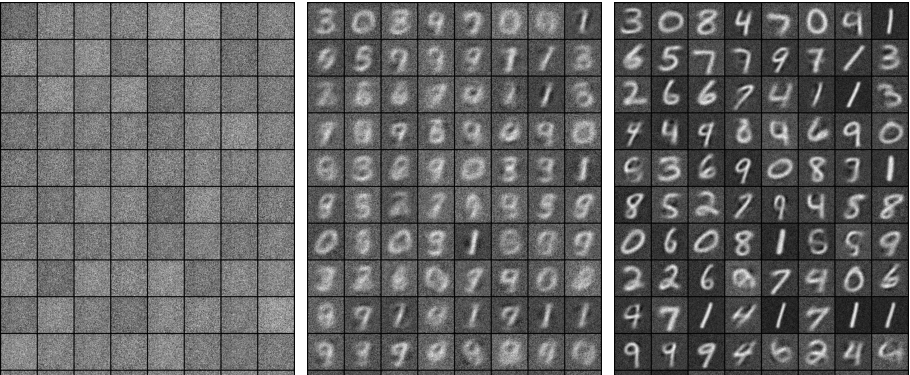
\includegraphics[width=0.41\columnwidth]{figures/mnist.pdf}
\label{fig:fashionmnist}	
}
\caption{The evolution of the particles through iterations on different datasets.}
\end{figure}

% \begin{figure}
% \begin{centering}
%   \setlength\tabcolsep{1pt}

% \begin{tabular}{cccc|c}
% $k=200$ & $k=2000$ & $k=10000$ & $k=40000$ & target\tabularnewline
% 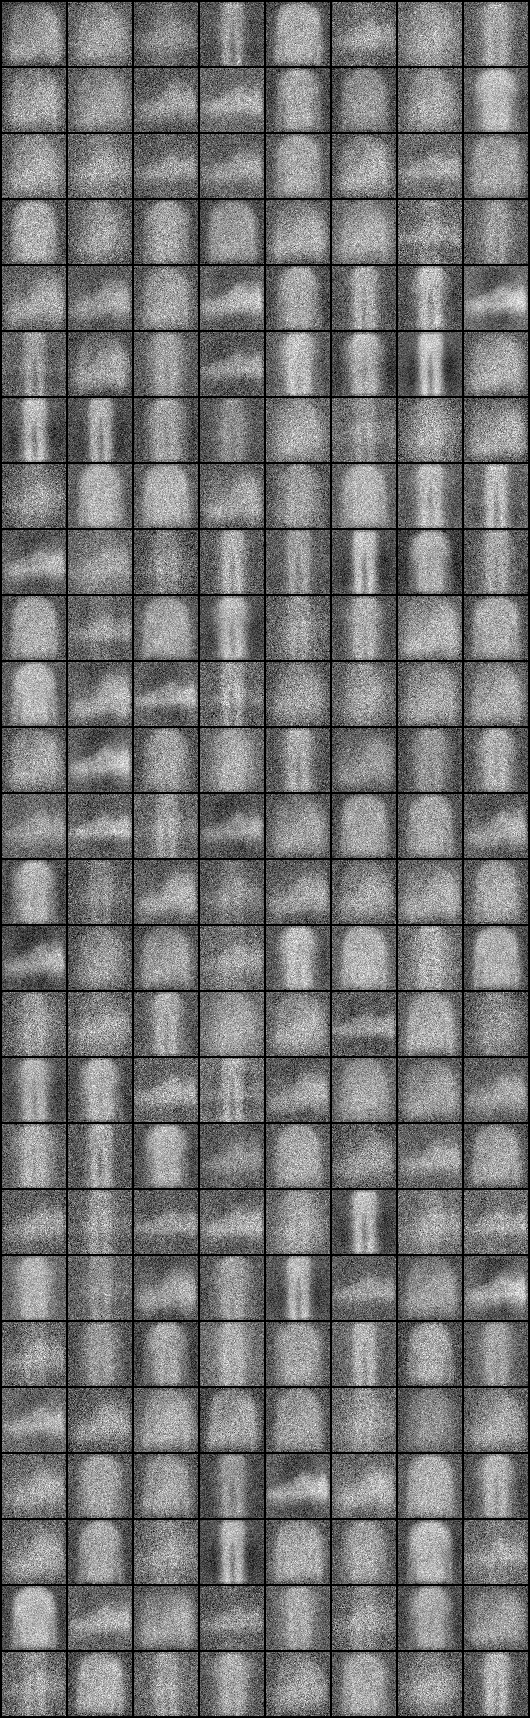
\includegraphics[height=6cm]{figures/FashionMNIST/image_200} & 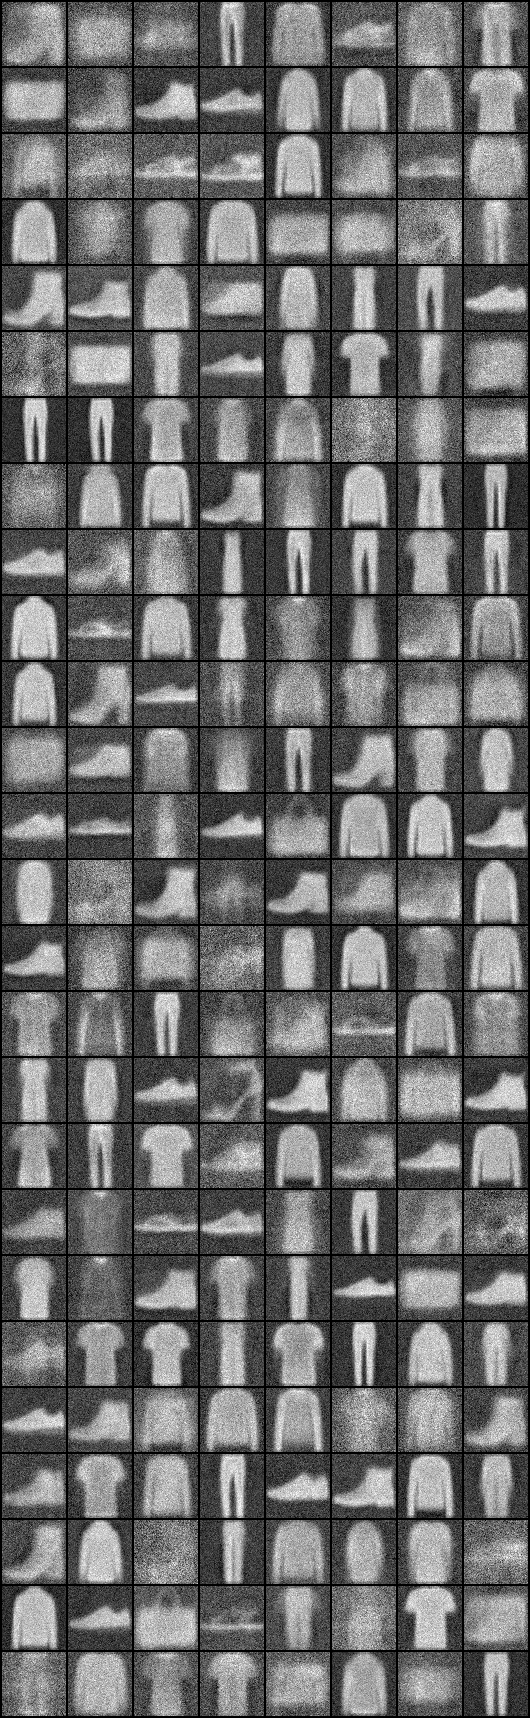
\includegraphics[height=6cm]{figures/FashionMNIST/image_2000} & 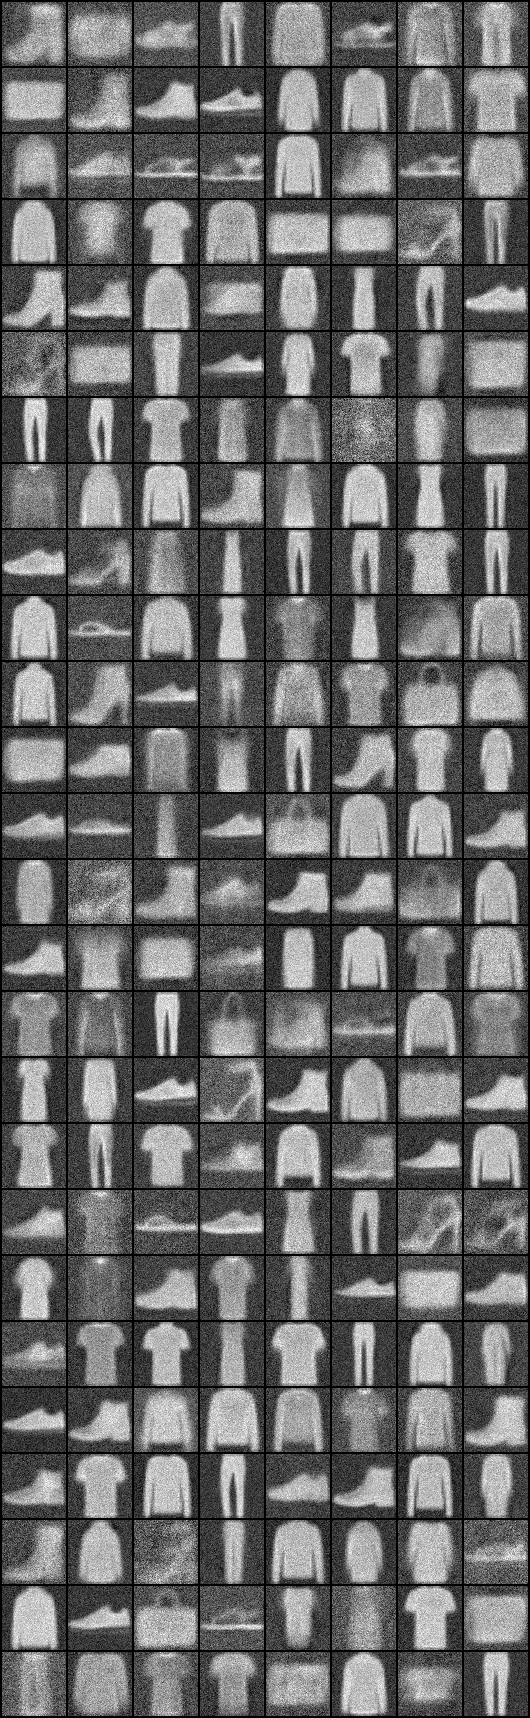
\includegraphics[height=6cm]{figures/FashionMNIST/image_10000} & 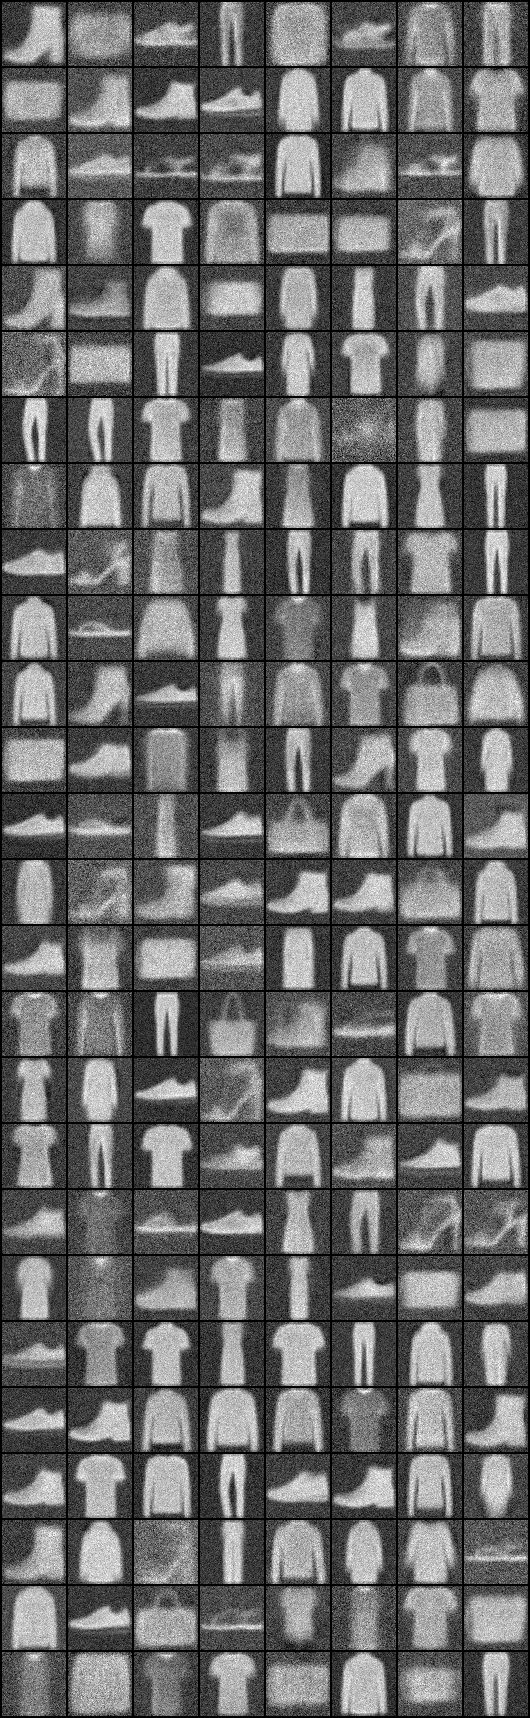
\includegraphics[height=6cm]{figures/FashionMNIST/image_38400} & 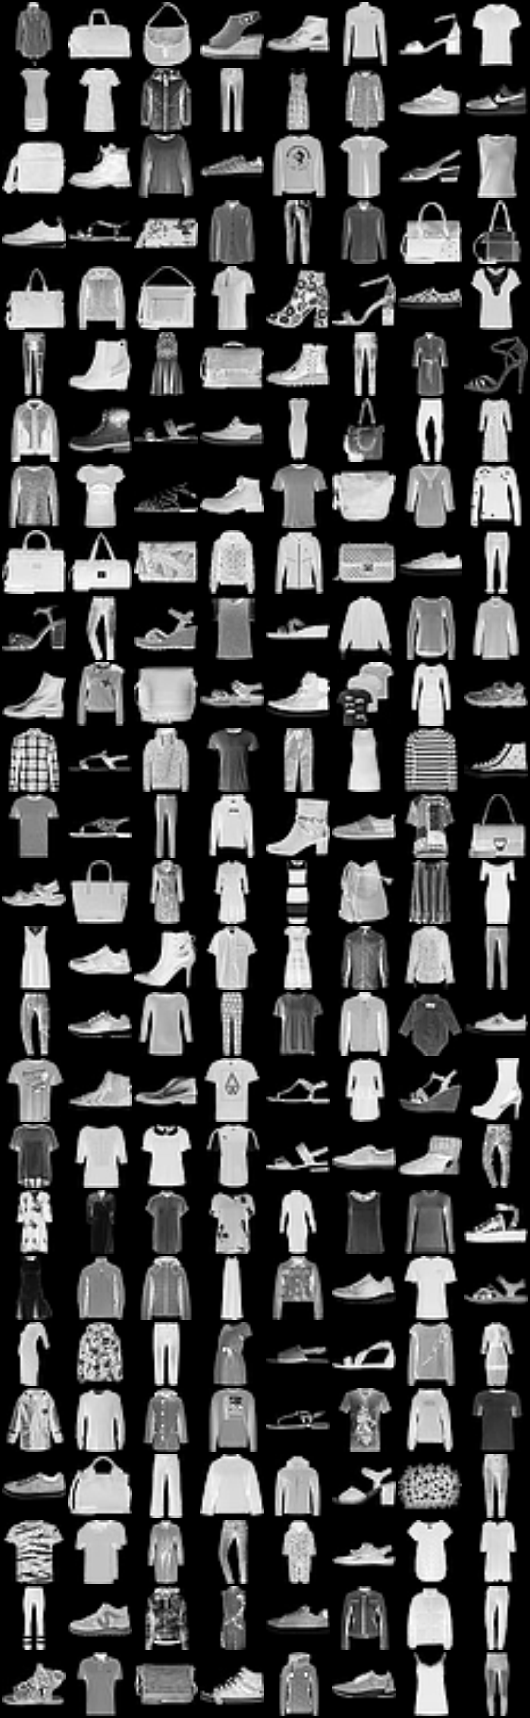
\includegraphics[height=6cm]{figures/FashionMNIST/dataset_example}\tabularnewline
% \end{tabular}
% \par\end{centering}
% \caption{Applying SWF on the Fashion MNIST dataset.\label{fig:fashionmnist}}
% \end{figure}

On figure \ref{fig:fashionmnist}, we can see that a few thousand iterations of SWF is sufficient to get generated samples that capture most features of the training data. We note however that we are currently missing generation of fine-grained textures. We also display the SW2 loss of this run along iterations. Interestingly, such an experiment requires around $1h$ of computing power for a laptop computer on CPU, to be compared with the important ressources required by many other generative models.

% \end{itemize}



% \begin{figure}
% \begin{subfigure}[t]{0.5\textwidth}
% \begin{centering}
% \setlength\tabcolsep{1pt}
% \begin{tabular}{ccc|c}
% $k=1$ & $k=7$ & $k=70$ & target\tabularnewline
% 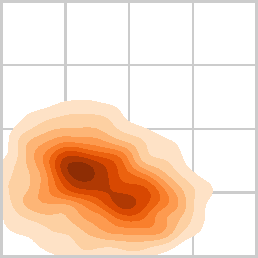
\includegraphics[width=2cm]{figures/toy_save/output_dist_k=1-crop.pdf} & 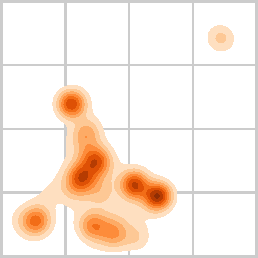
\includegraphics[width=2cm]{figures/toy_save/output_dist_k=20-crop.pdf} & 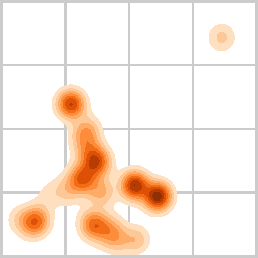
\includegraphics[width=2cm]{figures/toy_save/output_dist_k=70-crop.pdf} &  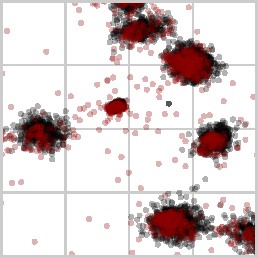
\includegraphics[width=2cm]{figures/scatter_output_particles_k=70-crop.pdf}\tabularnewline
% 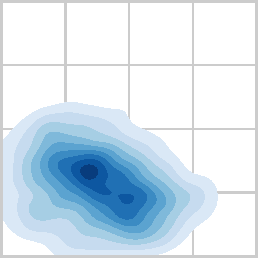
\includegraphics[width=2cm]{figures/toy_load/output_dist_k=1-crop.pdf} & 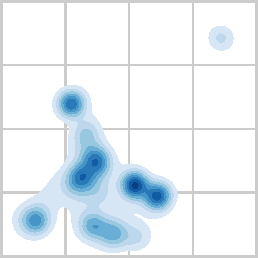
\includegraphics[width=2cm]{figures/toy_load/output_dist_k=20-crop.pdf} & 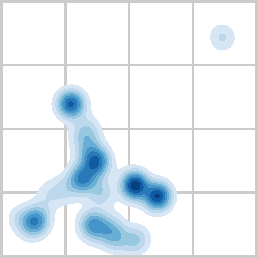
\includegraphics[width=2cm]{figures/toy_load/output_dist_k=70-crop.pdf} &  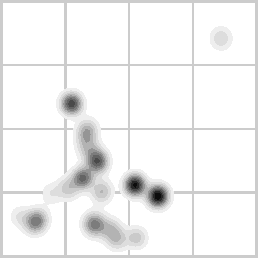
\includegraphics[width=2cm]{figures/target-crop.pdf}\tabularnewline
% \end{tabular}
% % \par
% \end{centering}
% \caption{Toy example.}
% \label{fig:toy_example}
% \end{subfigure}
% \end{figure}

% \begin{figure}
% \begin{centering}
% \setlength\tabcolsep{1pt}
% \begin{tabular}{cccccc}
% $\lambda=0$ & $\lambda=0.1$ & $\lambda=0.2$ & $\lambda=0.3$ & $\lambda=0.5$ & $\lambda=1$\tabularnewline
% 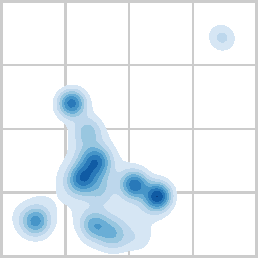
\includegraphics[width=2cm]{figures/supplementary/regularization/r0_output_dist_k=70-crop.pdf} & 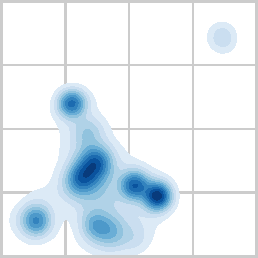
\includegraphics[width=2cm]{figures/supplementary/regularization/r01_output_dist_k=70-crop.pdf} & 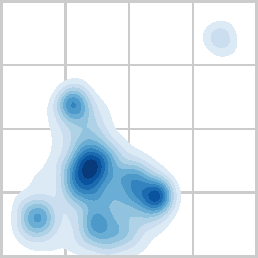
\includegraphics[width=2cm]{figures/supplementary/regularization/r02_output_dist_k=70-crop.pdf} &  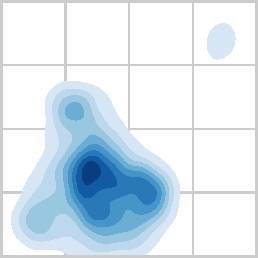
\includegraphics[width=2cm]{figures/supplementary/regularization/r03_output_dist_k=70-crop.pdf}&  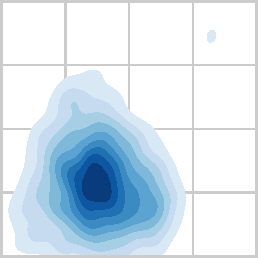
\includegraphics[width=2cm]{figures/supplementary/regularization/r05_output_dist_k=70-crop.pdf} &  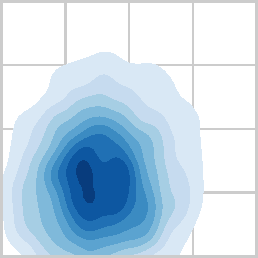
\includegraphics[width=2cm]{figures/supplementary/regularization/r1_output_dist_k=70-crop.pdf}
% \end{tabular}
% \par
% \end{centering}
% \caption{Influence of the regularization parameter $\lambda$. The higher $\lambda$, the more entropic the output distribution.\label{fig:lambda_supp}}
% \end{figure}








% \newcommand{\ww}{0.2}


% \begin{minipage}{\linewidth}
% \begin{minipage}{0.4\textwidth}
% \begin{figure}[H]
% \centering
% \begin{tabular}{ccc|c}
% $k=1$ & $k=7$ & $k=70$ & target\tabularnewline
% 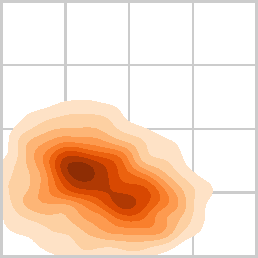
\includegraphics[width=0.1\columnwidth]{figures/toy_save/output_dist_k=1-crop.pdf} & 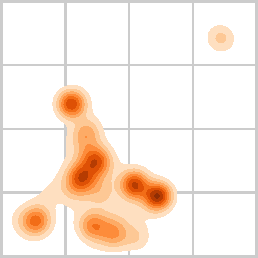
\includegraphics[width=0.1\columnwidth]{figures/toy_save/output_dist_k=20-crop.pdf} & 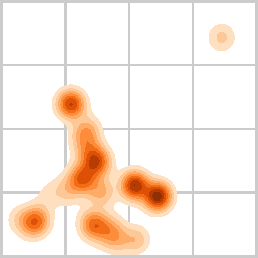
\includegraphics[width=0.1\columnwidth]{figures/toy_save/output_dist_k=70-crop.pdf} &  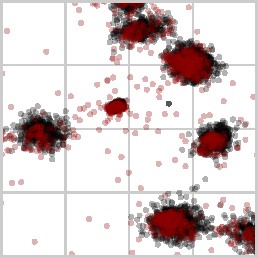
\includegraphics[width=0.1\columnwidth]{figures/scatter_output_particles_k=70-crop.pdf}\tabularnewline
% 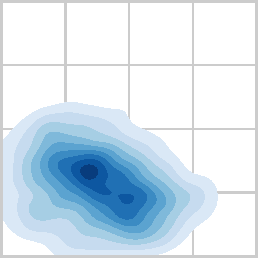
\includegraphics[width=0.1\columnwidth]{figures/toy_load/output_dist_k=1-crop.pdf} & 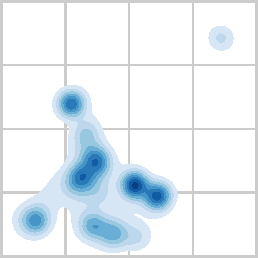
\includegraphics[width=0.1\columnwidth]{figures/toy_load/output_dist_k=20-crop.pdf} & 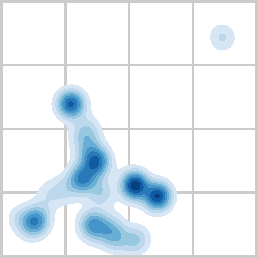
\includegraphics[width=0.1\columnwidth]{figures/toy_load/output_dist_k=70-crop.pdf} &  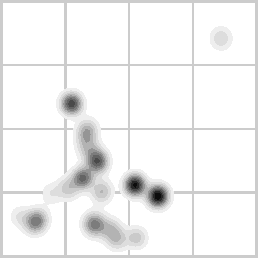
\includegraphics[width=0.1\columnwidth]{figures/target-crop.pdf}\tabularnewline
% \end{tabular}
% \par
% \caption{Toy example: training data $y_i$ consists in $50 000$ samples drawn from a Gaussian Mixture Model with $20$ components of random weights, covariances and locations. \textbf{Left:} Output distribution for learning (top) and testing (bottom) particles. \textbf{Right:} (top) Close-up of some generated samples in red superimposed with learning points in black. (bottom) Target distribution. $N_\theta=30$, $N=3000$, $h=1$, $\lambda=10^{-4}$.
% \label{fig:toy_example}}
% \end{figure}
% \end{minipage}
% %
% \begin{minipage}{0.49\textwidth}
% \begin{figure}[H]
% \centering
% \begin{tabular}{cccc|c}
% $k=2K$ & $k=20K$ & $k=10K$ & $k=40K$ & target\tabularnewline
% 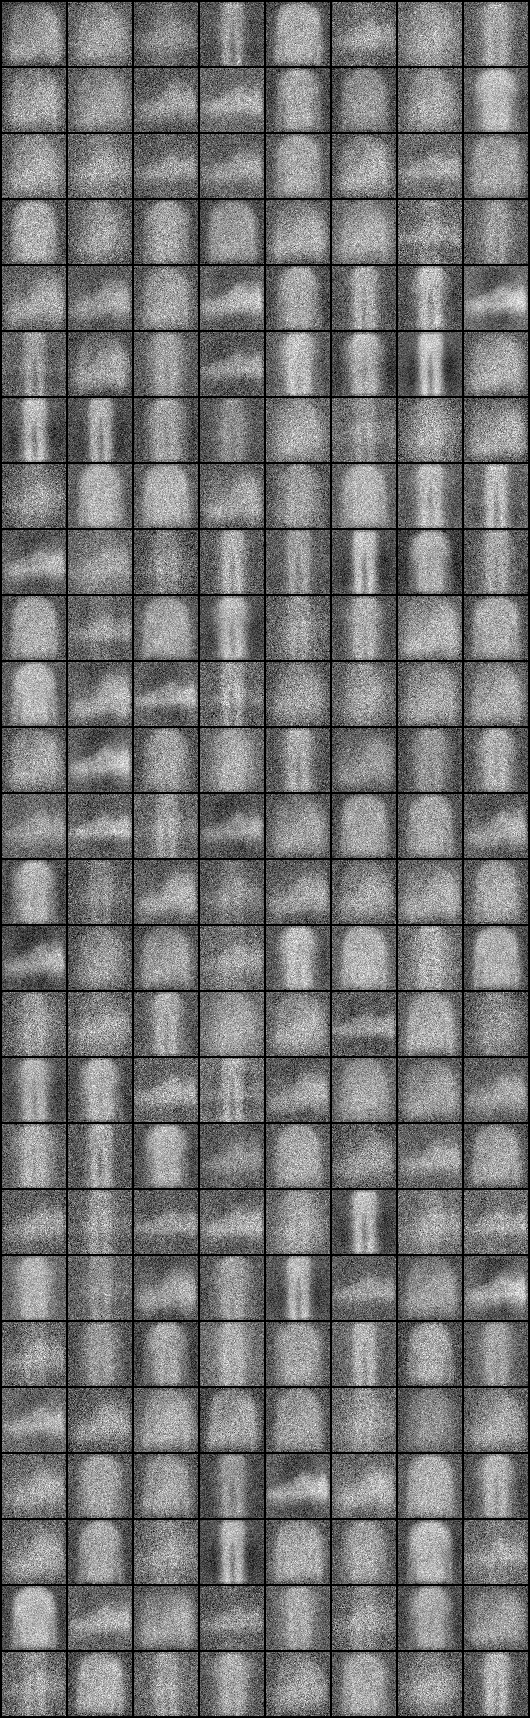
\includegraphics[width=\ww\columnwidth]{figures/FashionMNIST/image_200} & 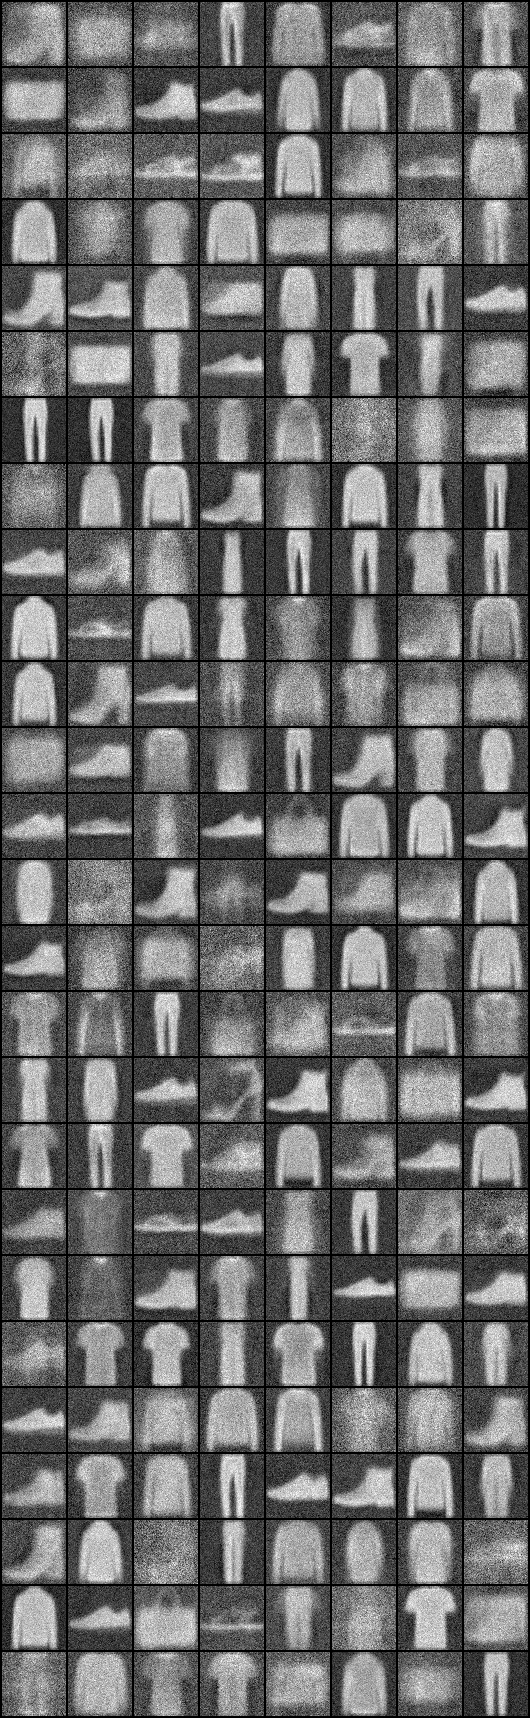
\includegraphics[width=\ww\columnwidth]{figures/FashionMNIST/image_2000} & 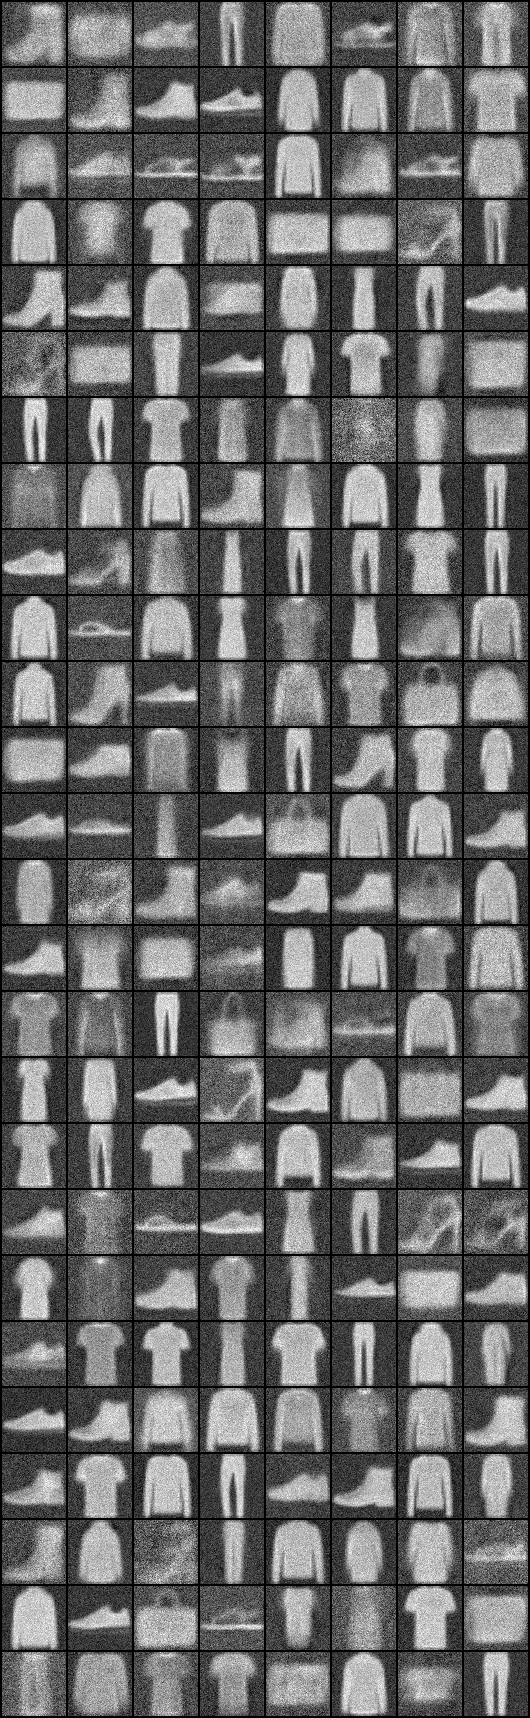
\includegraphics[width=\ww\columnwidth]{figures/FashionMNIST/image_10000} & 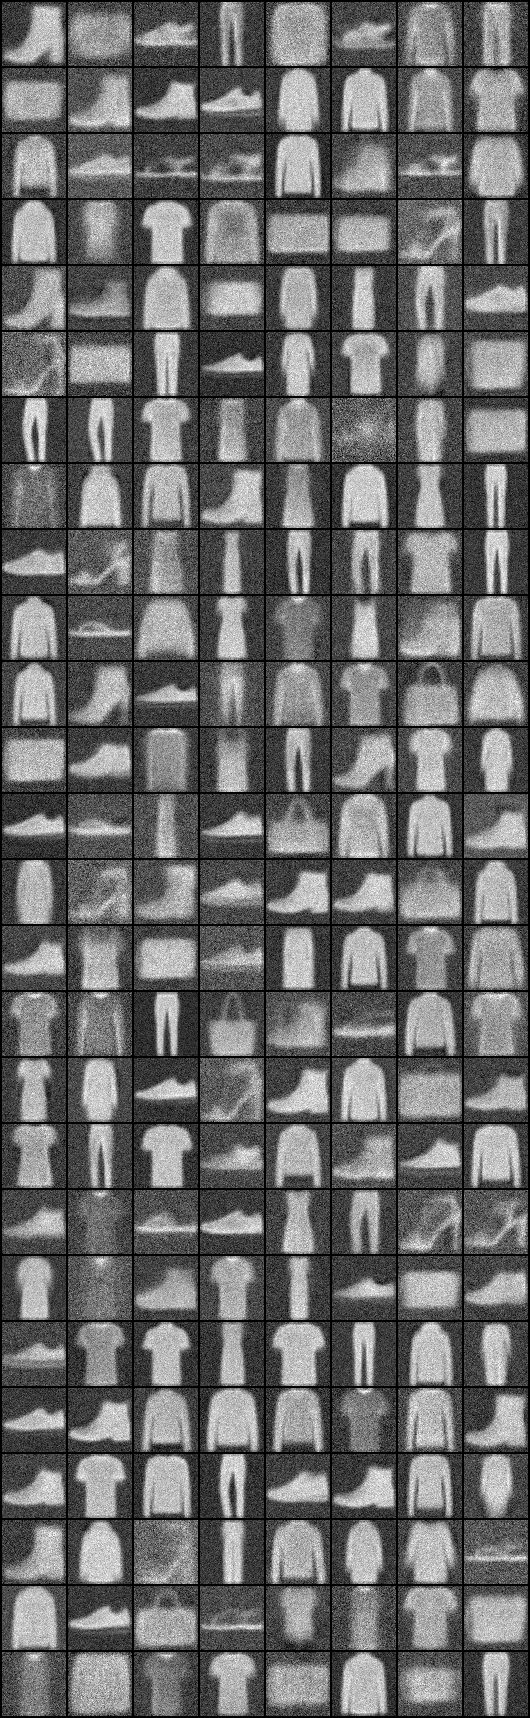
\includegraphics[width=\ww\columnwidth]{figures/FashionMNIST/image_38400} & 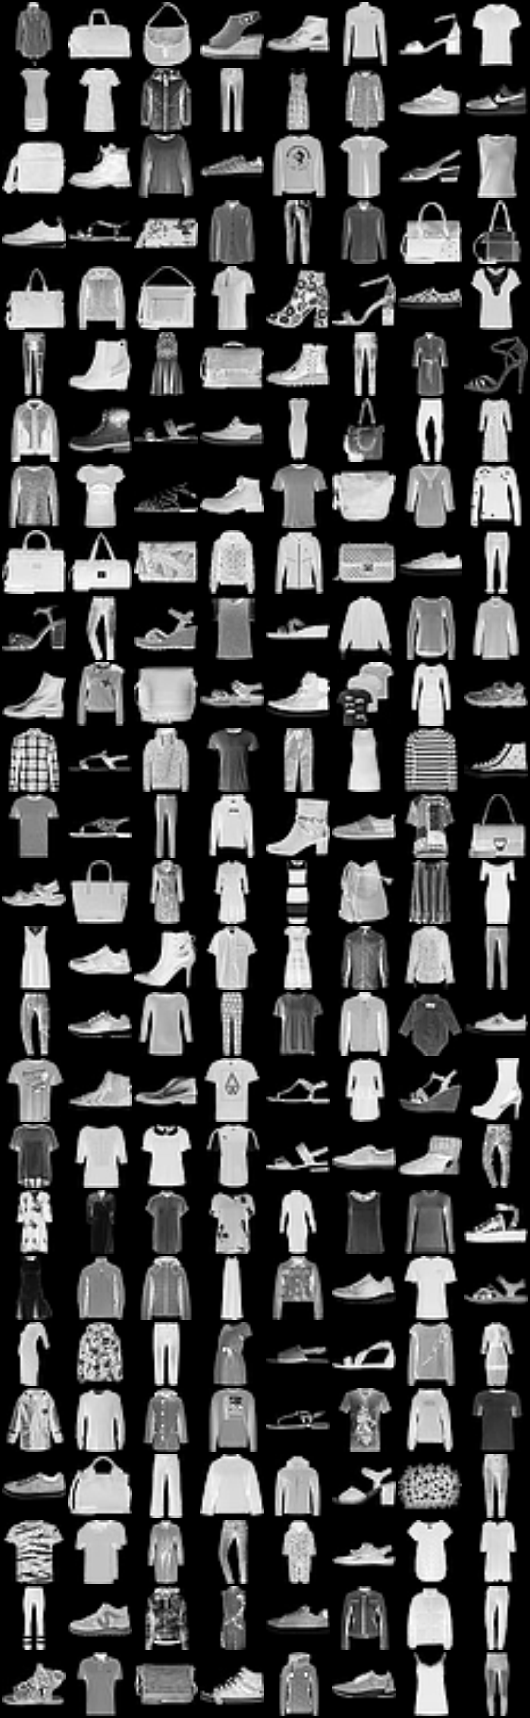
\includegraphics[width=\ww\columnwidth]{figures/FashionMNIST/dataset_example}\tabularnewline
% \end{tabular}
% \par
% \caption{Applying SWF on the Fashion MNIST dataset.
% \label{fig:fashionmnist}}
% \end{figure}
% \end{minipage}
% \end{minipage}
